\documentclass{exam}

\usepackage{amsmath,amssymb,amsfonts}
\usepackage{graphicx}
\usepackage{amsthm}
\usepackage[french]{babel}
\usepackage{enumitem}

\setlength{\topmargin}{-.5in} \setlength{\textheight}{9.25in}
\setlength{\oddsidemargin}{0in} \setlength{\textwidth}{6.8in}

\makeatletter
\def\gap#1{%
  \setbox\@tempboxa\hbox{{\color{white}#1}}%
  \@tempdima\wd\@tempboxa
  \rlap{\unhbox\@tempboxa}%
  \hb@xt@\@tempdima{\dotfill}%
}
\makeatother   

\theoremstyle{definition}
\newtheorem{exercice}{Exercice}

\begin{document}
\Large

\noindent{\bf Contrôle 1 (B) -- 1h. \hfill Première générale -- Groupe 2 \hfill 23/09/2024}
\vspace{5mm}
\noindent{\makebox[\textwidth]{Nom et prénom:\enspace\hrulefill}}

\begin{center}
\fbox{\fbox{\parbox{5.5in}{\centering
Répondez dans les espaces fournis. Si vous n'avez plus de place, continuez sur le verso.}}}
\end{center}

~\\



\medskip\hrule

\begin{exercice}[Calculer]
    \begin{enumerate}
    \item Pour chacune des suites suivantes, indiquer si elle est définie par une formule explicite ou par récurrence:
    \begin{enumerate}
        \item $u_n = 4n^2$
        
        \hrulefill
        \item $v_{n} = 5v_{n-1}$

        \hrulefill
        \item $w_{n} + 1 = n$
        
        \hrulefill
        \item $r_{n+1} = r_n - 5$

        \hrulefill
    \end{enumerate}
    
    \item Dans chaque cas, calculer les 3 premiers termes. Si la suite est définie par récurrence, prendre $-1$ pour valeur du premier terme. Par exemple, prendre $u_0 = -1$ si $(u_n)$ est définie par récurrence.% Remplissez le tableau ci-dessous.
    \end{enumerate}
    \begin{center}
        \framebox[1\textwidth]{\parbox{5.5in}{ \centering \underline{Réponse:}
        \vspace{18em}
        }}
    \end{center}

    %\begin{center}
    %\begin{tabular}{|c|c|c|c|c|} 
    % \hline
    % $n$ & $u_n$ & $v_n$ & $w_n$ & $r_n$\\
    % \hline\hline
    % 0 & \hspace{5em} & \hspace{5em} & \hspace{5em} & \hspace{5em} \\ 
    % \hline
    % 1 & \hspace{5em} & \hspace{5em} & \hspace{5em} & \hspace{5em} \\ 
    % \hline
    % 2 & \hspace{5em} & \hspace{5em} & \hspace{5em} & \hspace{5em} \\ 
    % \hline
    %\end{tabular}
    %\end{center}
\end{exercice}

\begin{exercice}[Modéliser]
    Soit $w_n$ la suite définie par son premier terme $w_0 = 1$ et les autres termes sont obtenus en ajoutant $1$ au double du terme précédent. Donner la relation de récurrence entre $w_{n+1}$ et $w_n$.
\end{exercice}
\begin{center}
    \framebox[1\linewidth]{\parbox{5.5in}{\centering \underline{Réponse:}
    \vspace{2em}
    }}
\end{center}

\begin{exercice}[Calculer]
    Dans chaque cas, déterminer, si possible, le sens de variation de la suite $(u_n)$ sur $\mathbb{N}$.

    \begin{enumerate}
        \item $u_n = 3n + 3$
        \item $u_n = 2n^2 - n + 1$
        \item $u_n = \frac{n+1}{n}$
        \item $u_0 = 1, u_{n+1} = -2u_n$
    \end{enumerate}
    
\end{exercice}

\begin{center}
    \framebox[1\textwidth]{\parbox{5.5in}{ \centering
    \underline{Réponse:}
    \vspace{29em}
    }}
\end{center}

\newpage
\begin{exercice}[Modéliser]
    Aujourd'hui, la valeur d'une certaine action en bourse est de 150€. En supposant qu'elle perd en valeur à hauteur de $1\%$ chaque jour, donner l'expression de la suite $u_n$ représentant sa valeur après $n$ jours.

    \begin{center}
        \framebox[1\textwidth]{\parbox{5.5in}{ \centering \underline{Réponse:}
        \vspace{4em}
        }}
    \end{center}
\end{exercice}

\begin{exercice}[Calculer]
    Pour chaque suite $(u_n)$ suivante, exprimez $u_{n+2}$ en fonction de $n$ lorsqu'elle est définie explicitement ou en fonction de $u_n$ lorsqu'elle est définie par récurrence.
    \begin{enumerate}
        \item $u_n = 2^{3n} - 3n$
        \item $\begin{cases} u_0 = 1\\ u_{n+1} = 11 u_n - 3\end{cases}$
    \end{enumerate}
    \begin{center}
        \framebox[1\textwidth]{\parbox{5.5in}{ \centering \underline{Réponse:}
        \vspace{25em}
        }}
    \end{center}
\end{exercice}

\begin{exercice}[Raisonner]
    On considère la suite $u$ définie par $u_n = 4n - 2$ pour tout $n \in \mathbb{N}$.
    \begin{enumerate}
        \item Calculer $u_0, u_1, u_2$.
        \item Montrer que la suite $u$ vérifie la relation de récurrence suivante: pour tout $n \in \mathcal{N}, u_{n+1} = u_n + 4$.
    \end{enumerate}
    \begin{center}
        \framebox[1\textwidth]{\parbox{5.5in}{ \centering \underline{Réponse:}
        \vspace{17em}
        }}
    \end{center}
\end{exercice}

\begin{exercice}[\textbf{Bonus}, Modéliser]
    Chez les abeilles, le mâle s'appelle le faux bourdon (\verb|fb|) il provient d'un oeuf non-fécondé.
    Un oeuf fécondé, donne naissance à une abeille femelle (\verb|af|).
    Ainsi une \verb|af| a deux parents (une \verb|af| et un \verb|fb|) alors qu'un \verb|fb| n'a pas de père.
    On a représenté ci-dessous, l'arbre généalogique d'un \verb|fb| sur trois générations.

    \begin{center}
        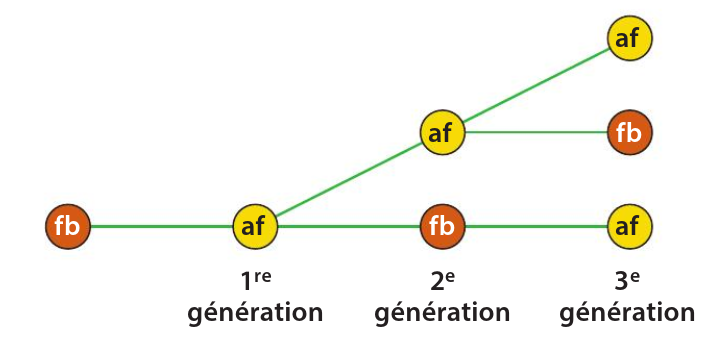
\includegraphics[width=0.6\textwidth]{Screenshot from 2024-09-16 11-50-56.png}
    \end{center}

    \noindent
    On note $a_n$ le nombre de descendants de ce faux-bourdon à la $n$-ième génération. On a donc $a_1 = 1, a_2 = 2, a_3 = 3$.

    \begin{enumerate}
        \item Donner les valeurs des termes $a_4, a_5$ et $a_6$. On pourra s'aider de l'arbre généalogique de l'énoncé, que l'on poursuivra.
    \end{enumerate}
    \begin{center}
        \framebox[1\linewidth]{\parbox{5.5in}{\centering \underline{Réponse:}
        \vspace{43em}
        }}
    \end{center}
    \newpage
    \begin{enumerate}[resume]
        \item Justifier que pour tout $n \geq 1$, on a $a_{n+2} = a_{n+1} + a_{n}$.
    \end{enumerate}
    \begin{center}
        \framebox[1\linewidth]{\parbox{5.5in}{ \centering \underline{Réponse:}
        \vspace{44em}
        }}
    \end{center}
\end{exercice}

\end{document}